\documentclass{article}

\usepackage[T1]{fontenc}
\usepackage[polish]{babel}
\usepackage[utf8]{inputenc}
\usepackage{lmodern}
\usepackage{indentfirst}
\usepackage{enumitem}
\usepackage{graphicx}
\graphicspath{ {./} }
\selectlanguage{polish}

\title{Markov Monster Chat}
\author{Adrian Zdanowicz}

\begin{document}

\maketitle


UWAGA: Poniższy dokument utworzony został w oparciu o wczesną koncepcję programu.
Niektóre z zawartych w nim założeń oraz opisywane sposoby użycia mogą
ulec zmianie w późniejszej fazie tworzenia projektu.


\section{Opis działania programu}

Program \textbf{Markov Monster Chat}, będący rozwinięciem projektu Markov Monster, to
narzędzie symulujące czat. Użytkownik dostaje do dyspozycji okno rozmowy z programem, który
odpowiada na każdą wiadomość i uczy się na podstawie tego, co pisze rozmówca z krwi i kości.


\section{Przebieg działania programu}

Przebieg działania programu dzieli się na etapy:

\subsection{Odczyt przygotowanego wcześniej pliku słownika}

Aby wirtualny rozmówca mógł zacząć rozmowę, posiadając już jakąś bazę zwrotów, \textbf{Markov Monster Chat} może przed rozpoczęciem rozmowy wczytać plik słownika. Zostaje on analizowany
i rozbity na łańcuchy Markova.

\subsection{Rozmowa}

Po przejściu pierwszego, opcjonalnego kroku, program rozpoczyna \textit{rozmowę} z użytkownikiem. Po wysłaniu wiadomości powitalnej, czeka on na odpowiedź użytkownika. Gdy
ta nastąpi, przesłana wiadomość jest analizowana i rozbijana na łańcuchy Markova tak, jak pliki
tekstowe przesyłane do poprzedniego projektu.


\section{Użycie programu}

Program \textbf{Markov Monster Chat} bazuje na interfejsie graficznym, dzięki czemu jest łatwy
w użyciu. Głównym elementem inferfejsu jest okno rozmowy z programem. Oprócz tego, udostępnione są zakładki, w których użytkownik może skonfigurować wirtualnego rozmówcę poprzez wczytanie mu bazy zwrotów z pliku słownika oraz wybór długości n-gramu, z którego budowane będą odpowiedzi.

Po zakończeniu rozmowy, istnieje możliwość zrzucenia wyuczonych słów do pliku słownika, dzięki
czemu każda następna rozmowa staje się bardziej różnorodna.


\section{Interfejs graficzny}

Interfejs graficzny programu prezentuje się następująco:

\bigskip
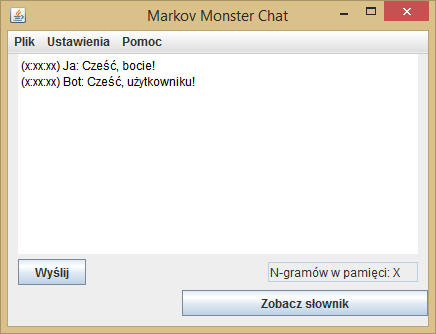
\includegraphics{mmchat}

\end{document}